\documentclass[12pt, a4paper]{article}
\usepackage[utf8]{inputenc}			% Für Umlaute
\usepackage[T1]{fontenc}			% Für richtige Schrift
\usepackage[ngerman]{babel}			% Für neue deutsche Rechtschreibung (Trennung)
\usepackage{color}
\usepackage{amsmath}
\usepackage{amssymb}
\usepackage{graphicx}
\usepackage{textcomp}				% Fürs Gradzeichen
\usepackage[square,numbers,sort]{natbib}
\usepackage{wrapfig}
\usepackage{url}
\usepackage{subfigure} 

\usepackage{scrpage2}				% Für Kopf- und Fußzeilen
\pagestyle{scrheadings}				% Für Kopf- und Fußzeilen
\clearscrheadfoot					% Für Kopf- und Fußzeilen

\renewcommand{\labelenumi}{(\alph{enumi})}
\renewcommand{\labelenumii}{(\roman{enumii})}
\chead{Pfadoptimierung für den 3D-Druck}
\cfoot{David Welsch, Ken Hasenbank}

\begin{document}
%\title{Wintersemester 2017/2018\\Motion Planning\\Prof. Horsch, Rudi Scheitler}
\author{David Welsch, Ken Hasenbank}
\title{Seminararbeit - Pfadoptimierung für den 3D-Druck}

\makeatother

\makeatletter
\begin{titlepage}
 \begin{center}
  {\LARGE Hochschule Darmstadt}\\
  {\large Fachbereich Informatik \\[3.5cm]}
	{\huge\bf Motion Planning}\\[0.8cm]
  {\LARGE Seminararbeit\\Pfadoptimierung für den 3D-Druck\\[3.5cm]}
 {\large David Welsch und Ken Hasenbank}\\[0.5cm]
25.01.2018\\[3cm]
\begin{center}
{\large\bf Dozenten}\\[0.6cm]
  {\large Prof. Dr. Thomas Horsch}\\[0.2cm]
  {\large Rudi Scheitler}
\end{center}
\end{center}
\end{titlepage}
\makeatother


\newpage
\tableofcontents

\newpage
\ofoot{\thepage}
\setcounter{page}{1}

\section{Einleitung}

Thema dieser Seminararbeit ist die Verringerung der Druckdauer beim 3D-Druck. Der 3D-Druck ist ein Verfahren, bei dem durch das Aufbringen mehrerer sehr dünner Schichten Material, meist in Form von Plastik (Filament), ein dreidimensionales Objekt erstellt werden kann. Durch diese Technik können sehr leicht am PC erstellte Modelle in die Realität umgesetzt werden, ohne dass hierfür aufwendige Arbeiten, wie Schweißen, Sägen oder Kleben nötig sind.

Beim 3D-Druck gibt es jedoch einige Besonderheiten. So kann der Druck nicht mit beliebig hoher Geschwindigkeit durchgeführt werden, da ansonsten das Ergebnis nicht zufriedenstellend ausfällt. Zudem entstehen beim Druck fast immer Übergangswege, wenn das Objekt nicht durchgehend gedruckt werden kann. Da diese Übergangspfade sehr häufig vorkommen und die Druckgeschwindigkeit festgelegt ist, liegt in der Minimierung der Übergänge das größte Potential bei der Verringerung der Druckzeit beim 3D-Druck.

Im Paper \textit{Trajectory planning for 3D printing: A revisit to traveling salesman problem} beschäftigen sich die Autoren \textit{Nuwan Ganganath, Chi-Tsun Cheng, Kai-Yin Fok und Chi K. Tse} \cite{Paper.2016} mit der Problematik der Wegfindung beim 3D-Druck. Inhalt dieses Papers ist zum einen die allgemeine Wegfindung, im Besonderen beschäftigen sich die Autoren jedoch damit, die Übergänge zu verbessern. Wir orientieren uns in dieser Seminararbeit an den angestrebten und beschriebenen Lösungen zur Reduzierung der Druckzeit.

Wir wollen untersuchen, inwiefern es uns gelingt, diese Verbesserung der Druckzeit selbst nachzustellen. Hierfür beschreiben wir zuerst die Problemstellung und untersuchen dann, wie sich das Problem abstrahieren lässt, um es theoretisch untersuchen zu können. Hierbei werden wir verschiedene Lösungsansätze vorstellen. Anschließend überführen wir unsere theoretischen Überlegungen in eine Demo-Applikation, welche die von uns gewonnenen Erkenntnisse und Lösungsansätze umsetzt. Hier ist das Ziel unseren Lösungsansatz auf eine vorhandene 3D-Druck-Datei (.gcode) anzuwenden, um eine Verringerung der Druckdauer zu erreichen. 

\newpage
\section{Problemstellung\label{kap:Problemstellung}}

Wie bereits in der Einleitung angedeutet wird beim 3D-Druck aus einem am PC konstruierten Modell ein reales Modell erstellt. Um ein am PC erstelltes Modell in eine für den 3D-Drucker verständliche Sprache zu übersetzen werden sogenannte Slicer-Programme eingesetzt. Diese berechnen aus dem Modell, häufig im .stl-Dateiformat, eine für den Drucker verständliche .gcode-Datei. Diese beinhaltet einzelne Code-Zeilen, welche Steuerkommandos für den Drucker enthalten. Die meisten dieser Kommandos sind Bewegungsanweisungen im Raum, welche vom Drucker durchgeführt werden sollen. Hierbei können zwei Bewegungen unterschieden werden, solche, in denen Filament aus der Düse gedrückt wird, und solche, in denen die Düse nur bewegt wird. Zur Unterscheidung dieser beiden Bewegungen später mehr.

Der Druck wird dann vom Drucker im Normalfall mit Hilfe von Plastik-Filament, welches in der Düse bei bis zu 250 Grad Celsius geschmolzen und mit einer Breite zwischen 0.3m und 1mm und einer Höhe zwischen 0.1 und 1mm pro Schicht aus der Düse gepresst wird, durchgeführt. Durch einen direkt an der Düse befestigten Lüfter wird das so geschmolzene Filament direkt wieder abgekühlt. Dadurch erhärtet das ausgegebene Filament direkt wieder und das Modell kann Schicht für Schicht aufgebaut werden.

Da ein Modell jedoch nur selten aus einem zusammenhängenden Strang gebildet werden kann, muss häufig pro Schicht das Drucken kurz unterbrochen werden, um an eine andere Stelle zu fahren. Deshalb muss grundsätzlich zwischen zwei verschiedenen Arten der Bewegung unterschieden werden:
\begin{itemize}
\item Druckbewegung\\
Diese Bewegung wird ausgeführt, wenn Filament aus der Düse gedrückt wird. Während dieser Bewegung wird das eigentliche Objekt erstellt. Bei dieser Bewegung wird die Geschwindigkeit von der Qualität des Druckers, dem Düsendurchmesser und der Schichthöhe festgelegt und kann zur Wahrung der Druckqualität nicht verändert werden.
\item Übergangsbewegung (im Folgenden \textit{Transition} genannt)\\
Bei Transitions handelt es sich um Bewegungen, welche von der Düse zurückgelegt werden müssen, um die nicht zusammenhängenden Teile eines Objektes zu drucken. Da diese Bewegungen keinerlei Einfluss auf das Druckergebnis haben, sollten diese so kurz wie möglich gehalten werden. Hier liegt deshalb das größte Verbesserungspotenzial. 
\end{itemize}
Schon die Notwendigkeit dieser Transitions an sich birgt ein großes Verbesserungspotential, da es je nach Beschaffenheit des zu druckenden Modells durchaus häufig zu solchen Bewegungen kommen kann. Zusätzlich dazu besitzen die verwendeten Slicer häufig ein vorgegebenes Muster an Bewegungen, welche häufig nicht optimal ist. So wird bei dem von uns verwendeten \textit{Simplify3D} (\url{https://www.simplify3d.com/}) immer zuerst die Außenhaut, dann die Füllung des Modells und zuletzt die eventuell benötigten Stützstrukturen gedruckt.\\
Diese vorgeschriebene Reihenfolge kann dazu führen, dass der Drucker häufig von einer Stelle zur anderen verfährt, obwohl dies nicht unbedingt nötig ist. So könnte es zum Beispiel besser sein, nach der Außenhaut zuerst eine Stützstruktur, dann die Füllung und zum Schluss den Rest der Stützstruktur zu drucken. Diese möglichen Verbesserungen wollen wir in dieser Seminararbeit untersuchen.

\subsection{Abstraktion}
\begin{wrapfigure}{L}{5.2cm}
	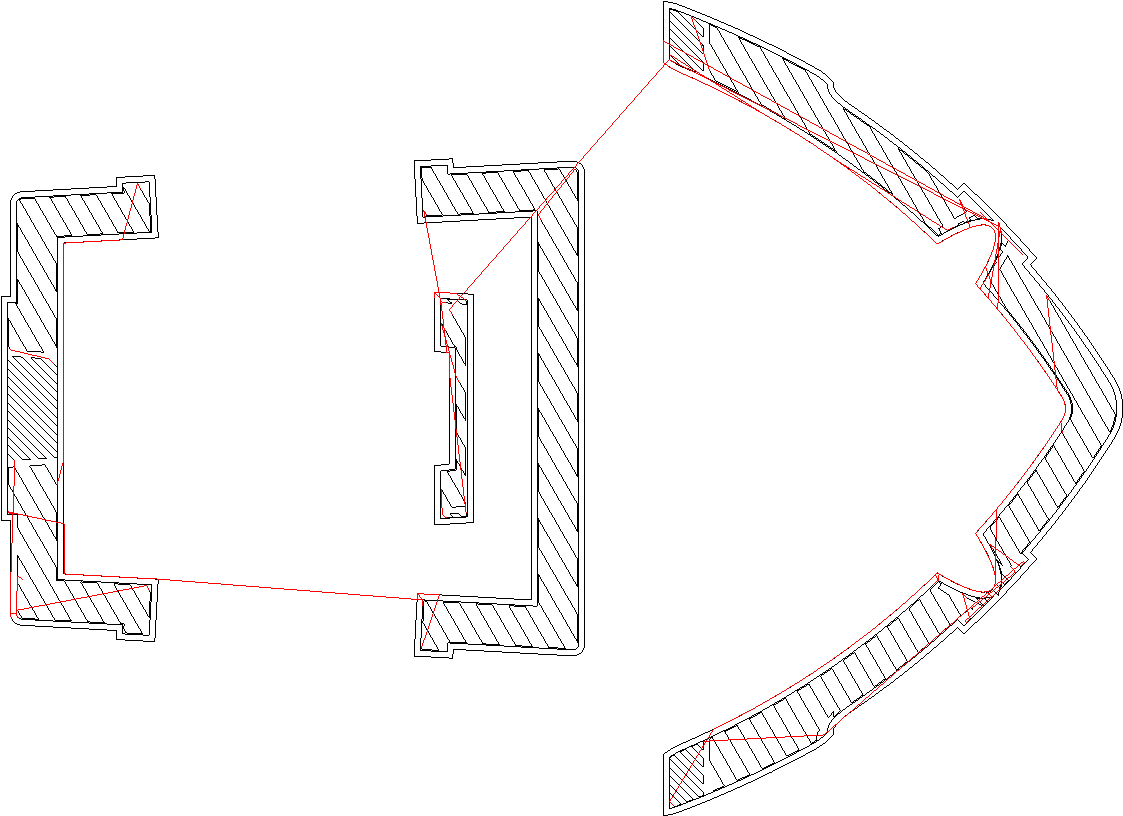
\includegraphics[width=5.1cm]{3DBenchylarge_gcode-224-Full-Transitions.png}
	\caption[Druckschicht nicht abstrahiert\newline Screenshot erstellt mit unserem PrintOptimizer]{Druckschicht nicht abstrahiert}
    \label{img:224FullTrans}
\end{wrapfigure}
Die in der .gcode-Datei vorhandenen Bewegungen können, wie bereits weiter oben beschrieben, in Druck- und Transitionpfade unterteilt werden. Hierfür lesen wir die .gcode-Datei ein und fassen zusammenhängende Druck- und Transitionpfade in Segmente zusammen. Diese Segmente haben einen Eintritts- sowie einen Austrittspunkt (Hit- und Leavepoint). Dazwischen findet die eigentliche Transition- oder Druckbewegung statt.
In Abbildung \ref{img:224FullTrans} ist der vollständige Druckpfad in schwarz, sowie die vom Slicer errechneten Transition-Pfade in rot zu sehen. Da wir die Druckbewegungen nicht verändern wollen und können, reduzieren wir alle Segmente auf ihre Hit- und Leavepoints. 
Dadurch abstrahieren wir alle Druckerbewegungen auf Übergänge von Druckpfad zu Transitionpfad und andersherum. In Abbildung \ref{img:224AbsTrans} ist die Abstraktion der Pfade auf Hit- und Leavepoints veranschaulicht. Auch hier sind die Druckpfade wieder in schwarz und die Transitionpfade in rot dargestellt.
\begin{wrapfigure}{R}{7cm}
	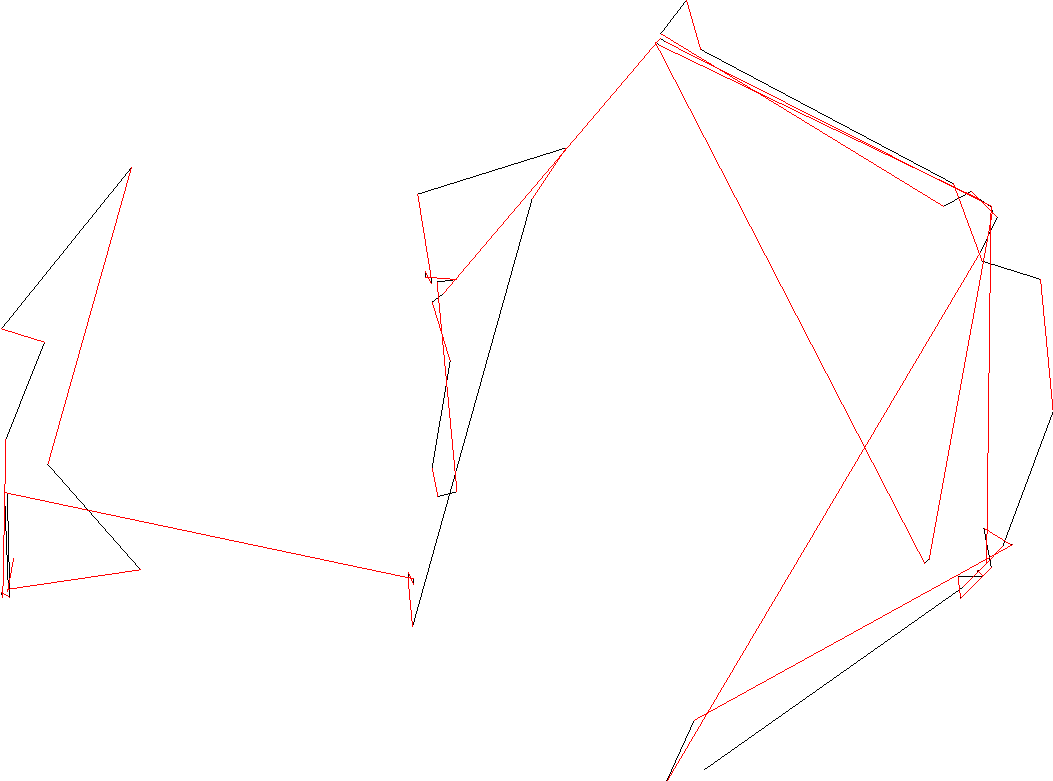
\includegraphics[width=6.8cm]{3DBenchylarge_gcode-224-Abstract-Transitions.png}
	\caption[Druckschicht abstrahiert\newline Screenshot erstellt mit unserem PrintOptimizer]]{Druckschicht abstrahiert}
    \vspace{-4.3cm}
    \label{img:224AbsTrans}
\end{wrapfigure} In dieser Ansicht sind jetzt nur noch die Hit- und Leavepoints der einzelnen Segmente sowie deren Verbindungen zu sehen. Ausgehend von dieser Abstraktion kann nun die eigentliche Optimierung stattfinden. Hierzu löschen wir alle Segmente, welche ausschließlich Transition-Pfade enthalten. So erhalten wir alle Segmente, abstrahiert auf Hit- und Leavepoints, welche für den Druck des Objekts nötig sind. Diese Segmente sind aus den oben genannten Gründen nicht veränderbar und sollen deshalb nicht mehr betrachtet werden. Die eigentliche Optimierung ist in Kapitel \ref{kap:Ergebnisse} beschrieben.\\

Trägt man die Hit- und Leavepoints der Drucksegmente nun auf einen Graphen auf, trifft man auf ein Problem, das dem \textit{Traveling-Salesman-Problem} sehr nahe kommt.
\vspace{3.5cm}
\subsection{Traveling Salesman \label{kap:TSP}}
\begin{wrapfigure}{L}{7cm}
	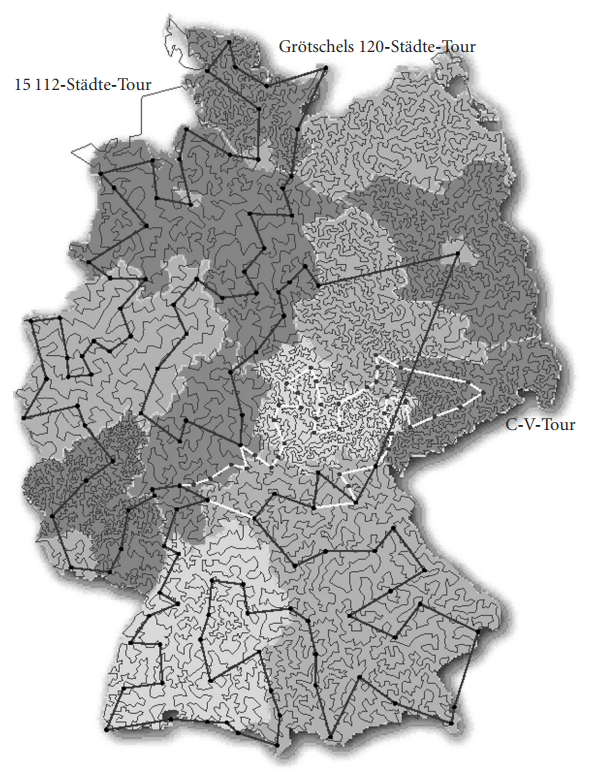
\includegraphics[width=6.9cm]{Groetschel.PNG}
	\caption[Darstellung des TSP\newline \cite{Groetschel.2005} ]{Darstellung des TSP}
    \label{img:TSP}
\end{wrapfigure}
Das \textit{Traveling Salesman Problem (kurz TSP)} ist eines der bekanntesten NP-harten Probleme der Informatik. Es beschriebt das Problem eines Handlungsreisenden, welcher bestimmte Städte auf einer Landkarte besuchen muss. Um dies möglichst effizient erledigen zu können, soll jede der Städte nur ein Mal besucht werden und der Weg zwischen den Städten soll möglichst kurz gewählt werden. Die optimale Lösung mehrere Traveling Salesman Probleme sind in Abbildung \ref{img:TSP} zu sehen. Die deutlichste Lösung, im Bild schwarz dargestellt, beschreibt eine Lösung einer 120-Städte-Tour durch Deutschland, welche im Jahre 1977 von Martin Grötschel errechnet wurde und damals den Weltrekord bedeutete. Die weiße Tour beschreibt die C-V-Tour, eine Tour welche bereits im Jahre 1832 im Reisehandbuch \textit{Handlungsreisende - wie er sein soll und was er zu thun hat, um Aufträge zu erhalten und eines glücklichen Erfolgs in seinen Geschäften gewiss zu sein - Von einem alten Commis-Voyageur} beschrieben war. Die schwarze, dünner gedruckte Tour beschreibt die 2001 gelöste 15.112-Städte Tour. Diese stellte wiederum einen Weltrekord dar und wurde an der Rice University in Houston und der Princeton University in Priceton berechnet \cite[vgl. Seite 111-112]{Groetschel.2005}.

Abstrahiert kann man das TSP also so formulieren, dass der kürzeste Weg zwischen mehreren Punkten gefunden werden soll, welche jedoch alle nur ein Mal besucht werden dürfen. So lässt sich das Problem auf sehr viele weitere Anwendungsfälle übertragen. \textit{Martin Grötschel} beschreibt in seinem Buch \textit{Schnelle Rundreisen: Das Travelling-Salesman-Problem} das TSP mit vielen Beispielen anschaulich \cite[Seite 93-129]{Groetschel.2005}.\\


In diesem Buch wird zudem eine mögliche Lösung des TSP beschrieben. Diese besteht darin, alle möglichen Wege zu enumerieren und dann den kürzesten auszuwählen. Dass diese Möglichkeit jedoch keine praktikable ist, beschreibt Grötschel ebenfalls. Das genannte Beispiel basiert auf der Bohrung einer Leiterplatine mit 18 Löchern. Der genutzte Algorithmus verwendet einen hamiltonischen Graphen, welcher die Rechenzeit verbessern soll:

\begin{quote}
,,Es braucht auf einem Dell PC mit 2 GB Speicher und mit
zwei Intel Pentium 4 Prozessoren, die mit 3,2 GHz getaktet sind, eine Gesamtrechenzeit
von 15.233 Minuten und 42,78 Sekunden, also nicht ganz 11 Tage, um [eine Lösung für] das 18-Löcher-Bohrproblem mit
max-Entfernung zu erzeugen.``  \cite[S. 108]{Groetschel.2005}
\end{quote}
Einige Zeilen später beschreibt er, dass die Komplexität dieses Algorithmus sehr schnell steigt:

\begin{quote}
,,Bedenkt man, dass man zur Lösung eines 25-Städte-Problems mit dieser Enumerationsmethode
eine Zeit benötigt, die 18×19× ... ×24-mal so lang ist, dann
müsste unser Laptop um den Faktor 1,7 Milliarden schneller sein, wenn wir ein
25-Städte-TSP in rund ein bis zwei Wochen lösen wollten. Enumeration ist also
nicht praxistauglich, und wir müssen uns etwas Besseres überlegen.`` \cite[S. 109]{Groetschel.2005}
\end{quote}

Daraus lässt sich ableiten, dass das Traveling Salesman Problem nicht in polynomieller Zeit lösen lässt und man sich einfachere Lösungsansätze überlegen muss.

\subsection{Abwandlung vom Traveling Salesman}

Zurück zu unserem Problem. Betrachten wir bei unseren Segmente ausschließlich die Hit- und Leavepoints und dort wiederum nur die auf einer Druckschicht vorhandenen, entsteht ein zweidimensionaler Graph mit mehreren Punkten. Diese Punkte müssen alle genau ein Mal besucht werden, um diese Schicht des zu erstellenden 3D-Modells zu drucken. Dabei spielt die Reihenfolge des Drucks, also welcher der beiden Punkte als Hit- und welcher als Leavepoint verwendet wird, keine Rolle. Der entstehende Graph kann also als ungerichteter Graph interpretiert werden. Der Unterschied zum TSP besteht jedoch darin, dass die einzelnen Punkte nicht gleichzeitig Eintritts- und Austrittspunkt sind, so wie dies beispielsweise bei zu besuchenden Städten normalerweise abstrahiert wird. Diese Besonderheit muss bei bei der Umsetzung der Algorithmen zur Lösung des TSP beachtet werden, stellt jedoch kein grundsätzliches KO-Kriterium zur Verwendung dieser Algorithmen dar, da sich diese auf diesen Spezialfall anpassen lassen.

Ein weiterer Unterschied zum normalen TSP besteht darin, dass im Pfad der Startpunkt nicht dem Endpunkt entsprechen muss, sondern beliebig gewählt werden kann. Die einzige Voraussetzung ist, dass der Endpunkt der vorherigen Druckschicht gleichzeitig der Startpunkt der aktuellen Druckschicht darstellt \cite[vgl. Kapitel III]{Paper.2016}.
Im Paper wird zudem als weiterer Unterschied genannt, dass nicht die Pfadlänge, sondern die Transition-Time verringert wird. Da jedoch eine Pfadverkürzung auch eine Verringerung der Transition-Zeit mit sich bringt und die normalerweise in einem 3D-Drucker verbauten Stepper-Motoren keine sehr lange Beschleunigungsphase haben, stellen wir unsere Berechnungen auf der Grundlage der Pfadlängen an.

\section{Lösungsansätze \label{kap:Lösungsansätze}}
Zur perfekten Lösung jedes TSP gibt es keinen Algorithmus, da das TSP zu den NP-harten Problemen gehört. Dies bedeutet, dass eine optimale Lösung nicht in polynomieller Zeit errechnet werden kann. Die Lösung eines TSP wird deshalb durch Optimierungsverfahren näherungsweise berechnet. Um eine ideale Lösung zu finden, muss jede erstellte Lösung mit allen anderen verglichen werden, um herauszufinden, ob die ermittelte Lösung ideal ist. Dies erfordert jedoch sehr viel Rechenaufwand, wie bereits in Kapitel \ref{kap:TSP} beschrieben. Deshalb wird häufig eine sogenannte \textit{Heuristik} verwendet, welche nicht den Anspruch hat, eine optimale Lösung zu finden, sondern sich mit einer Lösung zufrieden gibt, wenn diese in einer akzeptablen Zeit errechnet werden kann \cite[S. 113]{Groetschel.2005}. Drei dieser Heuristiken wurden im von uns untersuchten Paper zur Pfadplanung genutzt \cite[vgl. Kapitel III]{Paper.2016}. Diese sollen im Folgenden vorgestellt werden.

\subsection{Random Selection}
Beim \textit{Random Selection} Ansatz wird, wie der Name schon sagt, von einem gegebenen Startpunkt aus immer ein zufälliger nächster Punkt ausgewählt. Konkret geht der Algithmus so vor, dass zuerst alle Knoten in ein Set gespeichert werden. Ausgehend von einem Startpunkt wird dann ein Punkt aus diesem Set ausgewählt und aus dem Set gelöscht. Dieser Ablauf wird so lange fortgeführt, bis das Set leer ist. Die Knoten werden dann in umgekehrter Reihenfolge abgelaufen, um daraus einen Pfad zu erstellen. Im vorliegenden Paper wird dieser Ansatz genutzt, um die anderen untersuchten Algorithmen zu evaluieren.

\subsection{Nearest Neighbor Selection}
Der \textit{Nearest Neighbor Selection}-Algorithmus arbeitet ähnlich wie der \textit{Random Selection}-Algorithmus. Jedoch wird bei jedem Schritt geschaut, welcher Knoten am nächsten vom aktuellen Leavepoint entfernt ist. Da es beim 3D-Druck keine Rolle spielt, in welche Richtung gedruckt wird, können alle Hitpoints auch als Leavepoints und umgekehrt betrachtet werden. Dadurch wird im Gegensatz zum \textit{Random Selection}-Algorithmus sehr wahrscheinlich eine Verbesserung zu bemerken sein, da der Algorithmus einer gewissen Logik folgt.

\subsection{Christofides Algorithmus}
Der \textit{Algorithmus des Christofides} beschreibt eine Lösung, die höchstens die doppelte Länge der optimalen Lösung aufweist. Dies lässt sich durch mehrfache Anwendung der Dreiecksungleich zeigen. Dieser Beweis soll jedoch nicht Teil dieser Seminararbeit sein. 
Der Algorithmus arbeitet so, dass zuerst aus dem gegebenen Graphen ein minimaler Spannbaum (T) erstellt wird. Dann werden die Knoten ausgewählt, die eine ungerade Anzahl an Verbindungen besitzen. Diese bilden einen neuen Graphen G.  Auf diesem neuen Graphen wird ein perfektes Matching (M) gesucht. Die Kanten dieses Matchings werden zum Spannbaum T hinzugefügt. Per Definition ist dieser Graph dann eulersch. Dadurch kann eine \textit{Eulertour} auf diesem Graphen berechnet werden. Anschließend kann basierend auf dieser Tour und einem beliebigen Startpunkt ein Hamiltonkreis konstruiert werden. Dabei werden alle bereits besuchten Knoten durch den nächsten nicht besuchten Knoten ersetzt. \cite[vgl.]{Chr76}

\newpage
\section{Optimierungsansatz \label{kap:Heuristik}}
Ein zusätzlicher Ansatz zur Optimierung besteht darin, sogenannte \textit{k-opt Heuristiken} zu nutzen. Diese Heuristiken haben gemeinsam, dass sie bereits vorhandene Lösungen weiter verbessern. Sie können selbst also keine Lösung für das TSP herstellen sondern arbeiten auf einer Lösung, welche vorher beispielsweise von einem der in Kapitel \ref{kap:Lösungsansätze} beschriebenen Algorithmen erstellt wurde. Diese Algorithmen gehören zu der Klasse der \textit{Post-Optimization-Algorithmen}. Im Folgenden wird die \textit{2-opt-Heuristik} beschrieben.

Diese funktioniert so, dass sie sich überkreuzende Pfade sucht und diese tauscht. Dann wird geprüft, ob der neu entstandene Pfad weiterhin valid ist. Ist dies der Fall, wird der neu erstellte Pfad als neuer Pfad gespeichert. Bringt die Verbesserung keine Vorteile, wird der vorherige Pfad nicht verändert. Da sich überkreuzende Pfade jedoch fast immer eine Verlängerung der Laufzeit bedeuten, birgt die Anwendung der 2-opt Heuristik in eigentlich allen Fällen Vorteile. Die wird auf im untersuchten Paper deutlich. In der Tabelle 1 am Ende des Papers \cite[TABLE I]{Paper.2016} sind die Ergebnisse der Pfadplanungsalgorithmen aufgeführt. Hier ist deutlich zu sehen, dass die 2-opt-Heuristik große Vorteile bringt. Hier schlägt sogar der \textit{Random Selection}-Algorithmus mit nachgelagerter Anwendung der 2-opt Heuristik den \textit{Nearest Neighbor Selection}-Algorithmus ohne die Anwendung der 2-opt Heuristik.

\newpage
\section{Ergebnisse und Demoprogramm \label{kap:Ergebnisse}}
Um das das beschriebene Problem zu veranschaulichen, haben wir uns als Ziel gesetzt, im Rahmen dieser Seminararbeit ein Demoprogramm zu entwickeln, welches eine zuvor erstellte .gcode-Datei einliest und einen der vorgestellten Lösungsansätze darauf anwendet. 

Nach Auswertung des Papers von \textit{Nuwan Ganganath, Chi-Tsun Cheng, Kai-Yin Fok und Chi K. Tse} \cite[vgl. Seite 290, TABLE I.]{Paper.2016} haben wir uns dazu entschieden, die \textit{Nearest Neighbour Selection} zu implementieren, da hier die signifikantesten Verbesserungen (im Verhältnis zum Aufwand) zu erwarten waren. 

\begin{figure}[h!]
	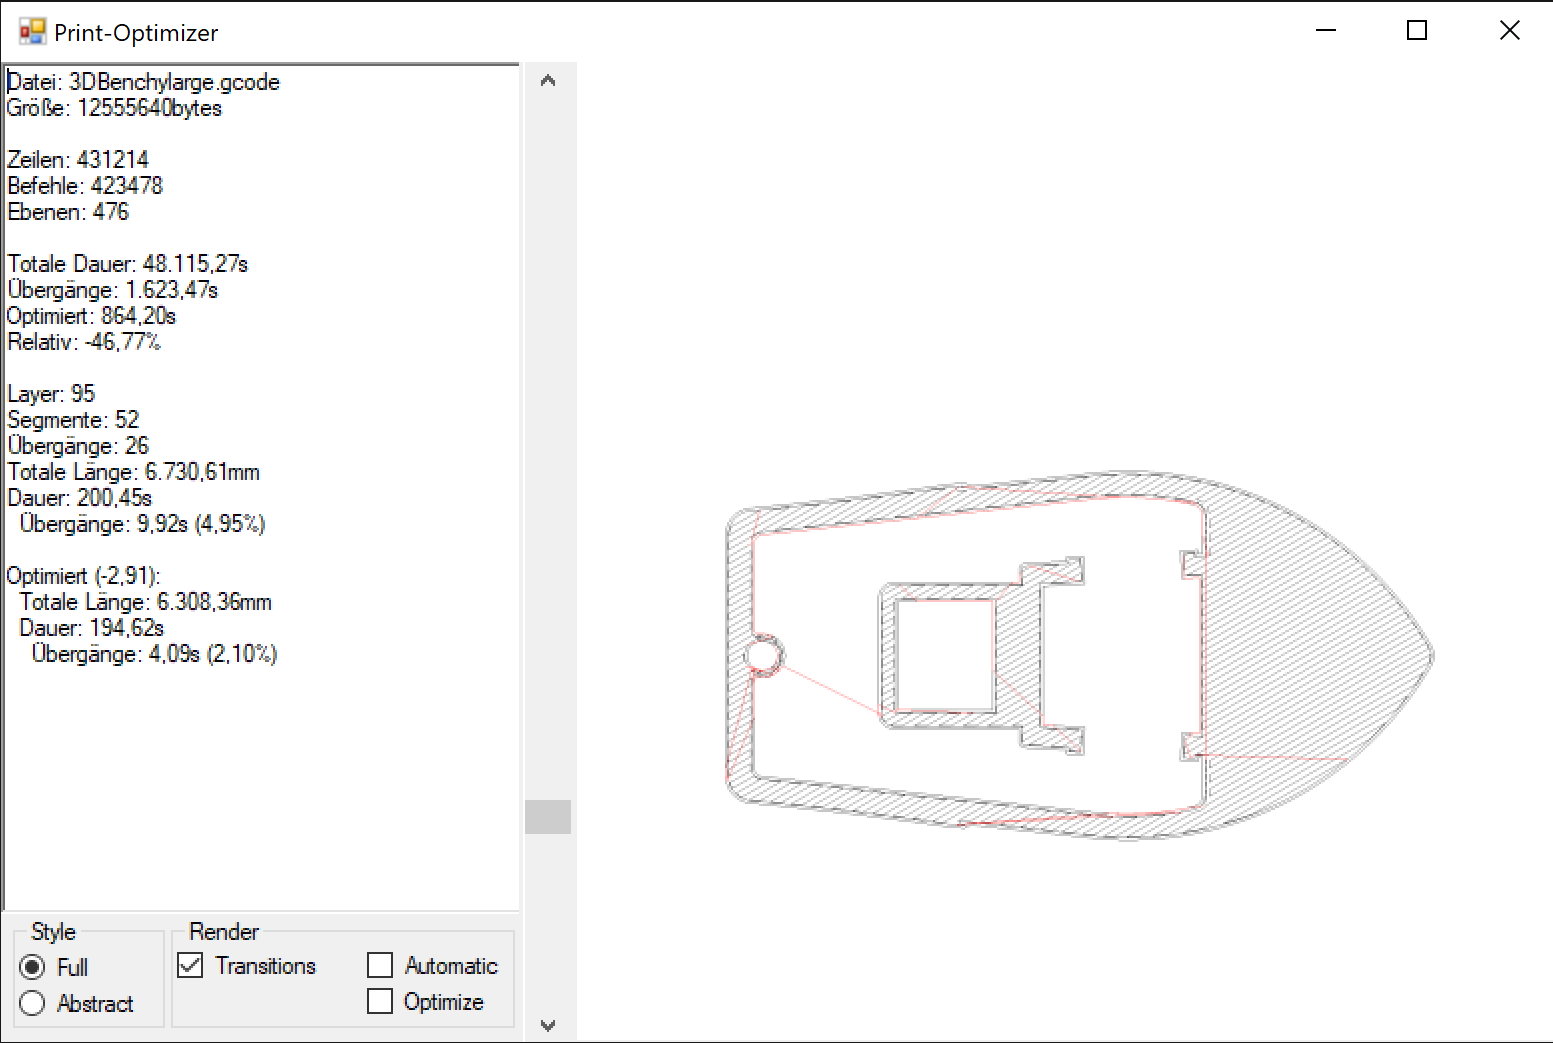
\includegraphics[width=\textwidth]{PrintOptimizer.PNG}
	\caption[PrintOptimizer\newline Screenshot erstellt mit dem Microsoft Snipping Tool]{PrintOptimizer}
    \label{img:PrintOptimizer}
\end{figure}
Als Ergebnis haben wir also ein Programm entwickelt, den \textit{PrintOptimizer} (Abbildung \ref{img:PrintOptimizer}), welches per Drag \& Drop .gcode-Dateien einlesen kann. Auf der linken Seite werden allgemeine Informationen zur Datei, sowie Informationen für eine spezifische Schicht angezeigt. Unterhalb dieser Informationen können verschiedene Einstellungen an den Renderer übergeben werden. Auf der rechten Seite wird das die aktuelle Schicht mit den aktuellen Einstellungen gerendert und angezeigt. Der Schichtindex kann über eine Scrollbar, welche die Informations-/ und Ansichtsfelder voneinander trennt, eingestellt werden.
Der Renderer stellt im Anzeigefenster alle Druckpfade mit einer schwarzen und alle Transitions mit einer roten Linie dar.
Folgende Einstellungen können verändert werden:
\begin{itemize}
  \item Style
  \begin{itemize}
  	\item Full \\
    Diese Einstellung weißt den Renderer an, die Druckpfade genau so zu zeichnen, wie sie später auch vom 3D-Drucker abgefahren werden. So kann man einfach erkennen, wie die im .gcode beschriebene Schicht später aussieht. (Siehe Abbildung \ref{img:224FullTrans})
  	\item Abstract \\
    Diese Einstellung weißt den Renderer an, nur die abstrahierten Druck-/ sowie Transitionpfade darzustellen. Das heißt, alle aneinanderhängenden Linien des gleichen Typs werden zu einer einzelnen Linie zusammengefasst. (Siehe Abbildung \ref{img:224AbsTrans})
  \end{itemize}
  \item Render
  \begin{itemize}
  	\item Transitions \\
    Diese Einstellung gibt an, ob die roten Transitions angezeigt werden sollen oder nicht.
  	\item Optimize \\
    Ist diese Option gewählt, so werden aus der aktuellen Schicht alle Transitions entnommen und mittels dem implementierten Algorithmus (\textit{Nearest Neighbour Selection}) durch neue ersetzt.
  	\item Automatic \\
    Nicht in jeder Schicht wird die Transitionzeit durch den angewendeten Algorithmus verringert. Ist die Option Automatic ausgewählt, wird der Renderer angewiesen, basierend auf der Transitionzeit, automatisch die originalen oder die optimierten Transitionpfade zu rendern.
  \end{itemize}
\end{itemize}
Über die Tastenkombination \textit{STRG + S} kann der Renderer angewiesen werden, das aktuelle Bild auf die Festplatte zu speichern. Bilder werden im aktuellen Ausführungsverzeichnis des PrintOptimizers abgelegt und mit dem Namen der eingelesenen Datei, sowie den aktiven Einstellungen benannt.

\begin{samepage}
Zum Testen haben wir uns von der Digital-Design-Sharing-Plattform Thingiverse (\url{https://www.thingiverse.com}) vier Objekte heruntergeladen, mithilfe von \textit{Simplify3D} in .gcode-Dateien umgewandelt.
\begin{itemize}
\item Benchy (\url{https://www.thingiverse.com/thing:2213891})
\item Schrodinky (\url{https://www.thingiverse.com/thing:2692916})
\item Electronics Case (\url{https://www.thingiverse.com/thing:1767285})
\item Sierpinski Pyramide (\url{https://www.thingiverse.com/thing:8711})
\end{itemize}
\end{samepage}

\begin{table}[h!]
 \begin{tabular}{|l|p{1.9cm}|l|p{2.1cm}|p{2.1cm}|}
 Model & Gesamte Druckzeit & davon Transitions & Optimierte Transitions & Prozentuale Verbesserung \\
 \hline
 Benchy & 48.115,27s & 1.623,47s (3,37\%) & 864,20s & -46,77\% \\
 \hline
 Schrodinky & 10.882,47s & 361,46s (3,32\%) & 246,93s & -31,68\% \\
 \hline
 Electronics Case & 27.805,44s & 3.231,78s (11,62\%) & 1.408,07s & -56,43\% \\
 \hline
 Sierpinski Pyramide & 13.901,25s & 2.782,18s (20,01\%) & 1.161,44s & -58,25\% \\
 \hline
 \end{tabular}
 
\caption{Testergebnisse}
\label{tbl:ergebnisse}
\end{table}

Aus Tabelle \ref{tbl:ergebnisse} ist zu entnehmen, dass die Transitionzeiten einen signifikanten Teil der gesamten benötigten Druckzeit ausmachen können. Der prozentuale Anteil der Transitionzeit gegenüber der tatsächlichen Druckzeit ist natürlich stark von den Modellen abhängig. Allerdings zeigen unsere Ergebnisse deutlich, dass bei den Transitionwegen ein enormes Verbesserungspotenzial besteht.

\newpage
\begin{samepage}
Die Folgenden Bilder sollen verdeutlichen, wodurch diese Verbesserungen zustande kommen:
\begin{figure}[h!]
    \subfigure[Druckpfad]{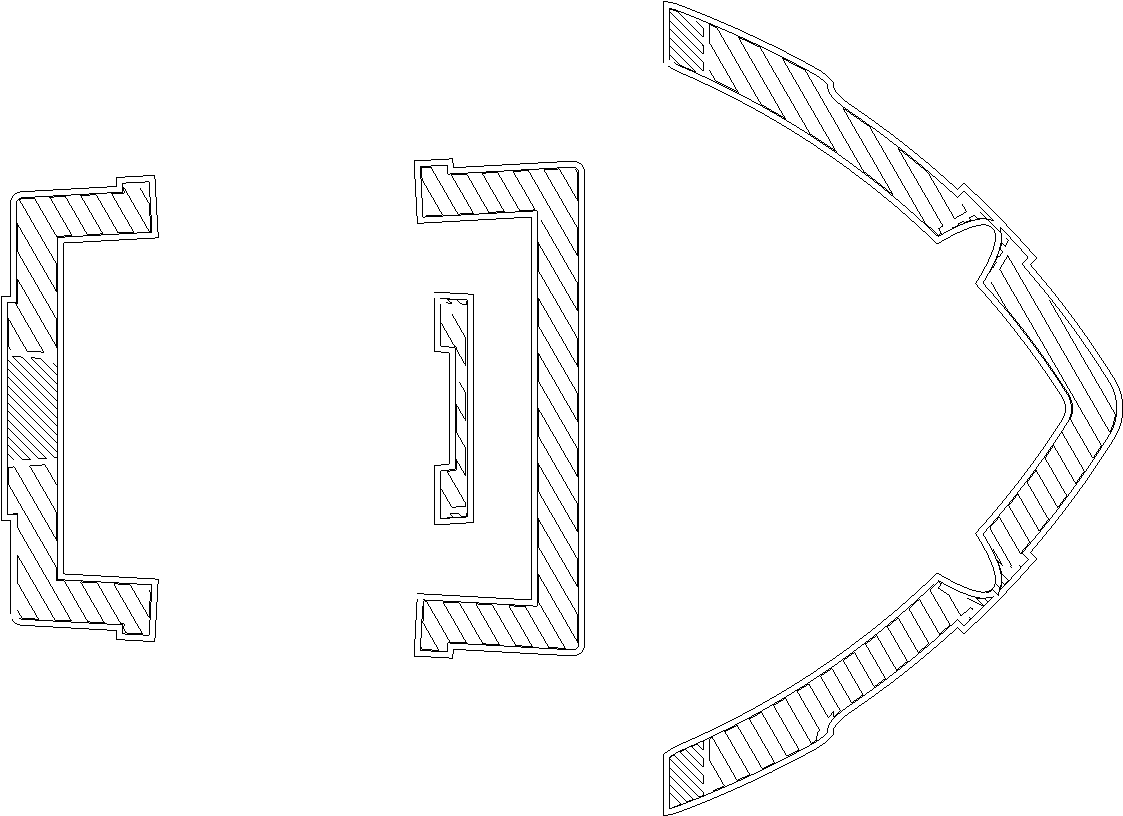
\includegraphics[width=0.32\textwidth]
    {3DBenchylarge_gcode-224-Full-NoTransitions.png}} 
    \subfigure[Abstraktion]{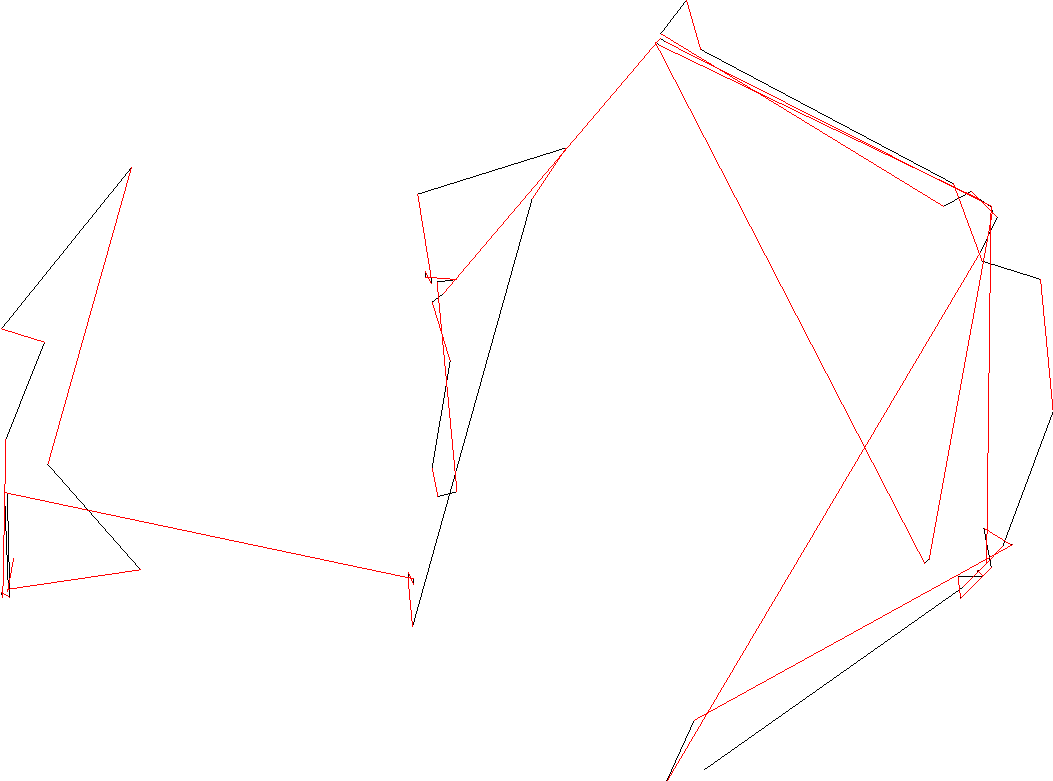
\includegraphics[width=0.32\textwidth]
    {3DBenchylarge_gcode-224-Abstract-Transitions.png}} 
    \subfigure[Optimiert - 7\%]{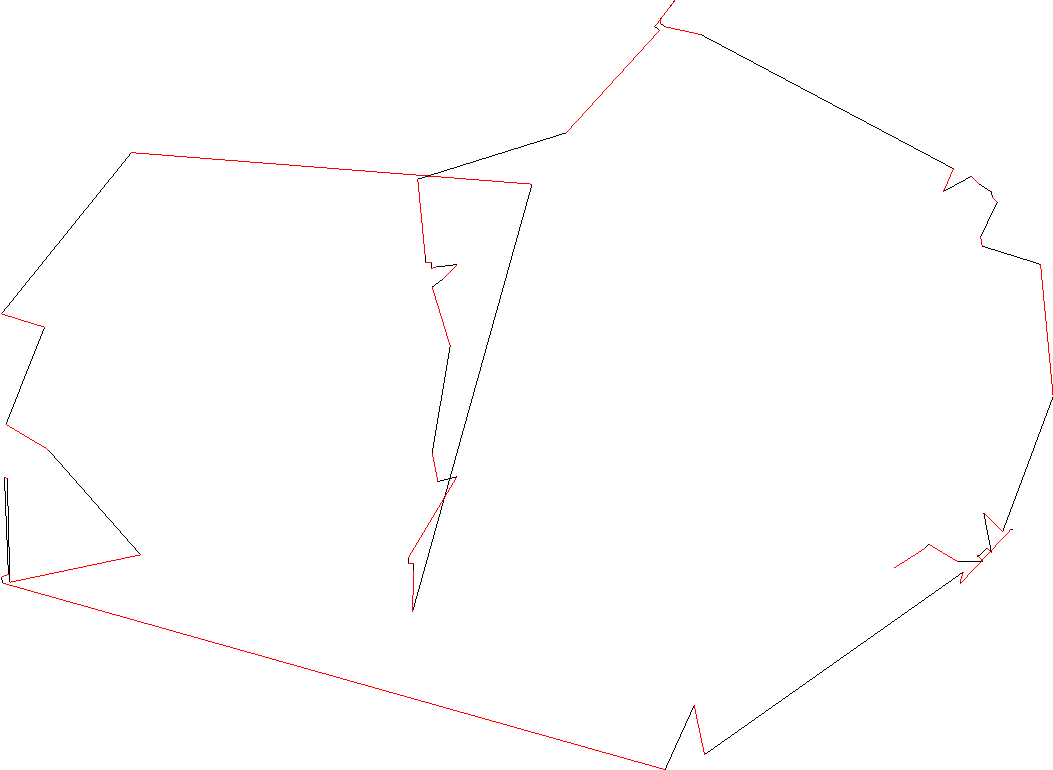
\includegraphics[width=0.32\textwidth]
    {3DBenchylarge_gcode-224-Abstract-Optimized-Transitions.png}} 
\caption[Schicht 224 aus dem Model \textit{Benchy}.\newline Screenshot erstellt mit unserem PrintOptimizer]{Schicht 224 aus dem Model \textit{Benchy}}
\label{img:benchy_layer}
\end{figure} 
\begin{figure}[h!]
    \subfigure[Druckpfad]{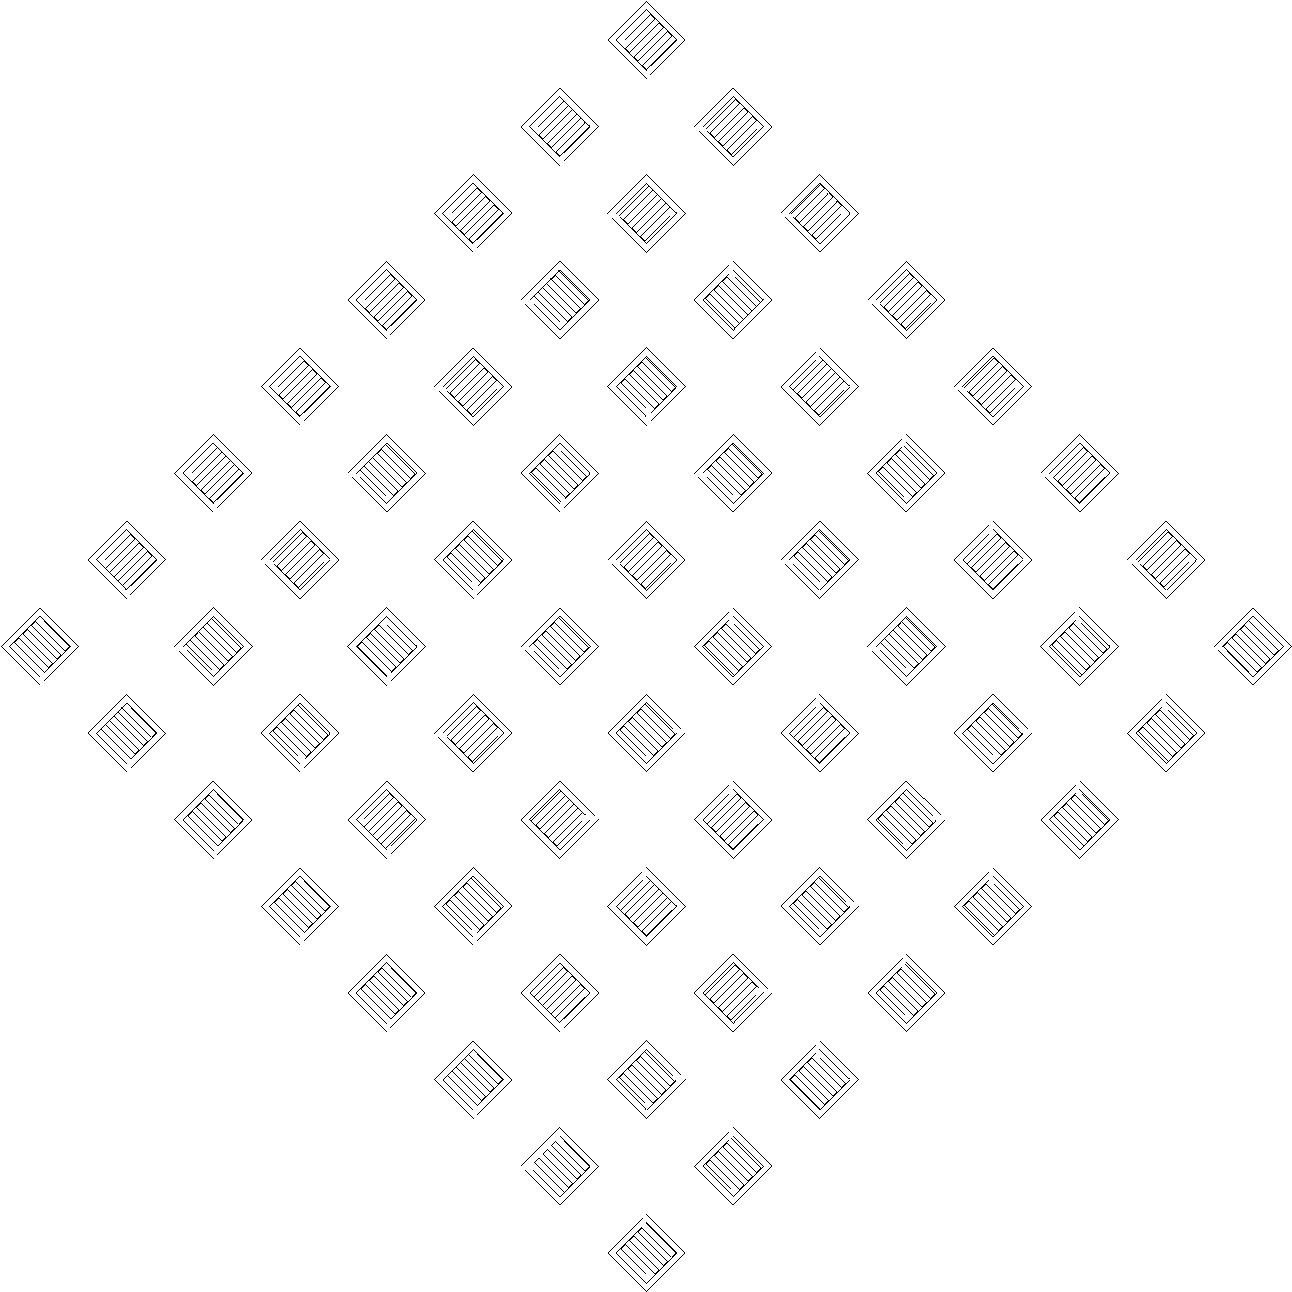
\includegraphics[width=0.32\textwidth]
    {sierpinski_print_yeahright_gcode-15-Full-NoTransitions.png}} 
    \subfigure[Abstraktion]{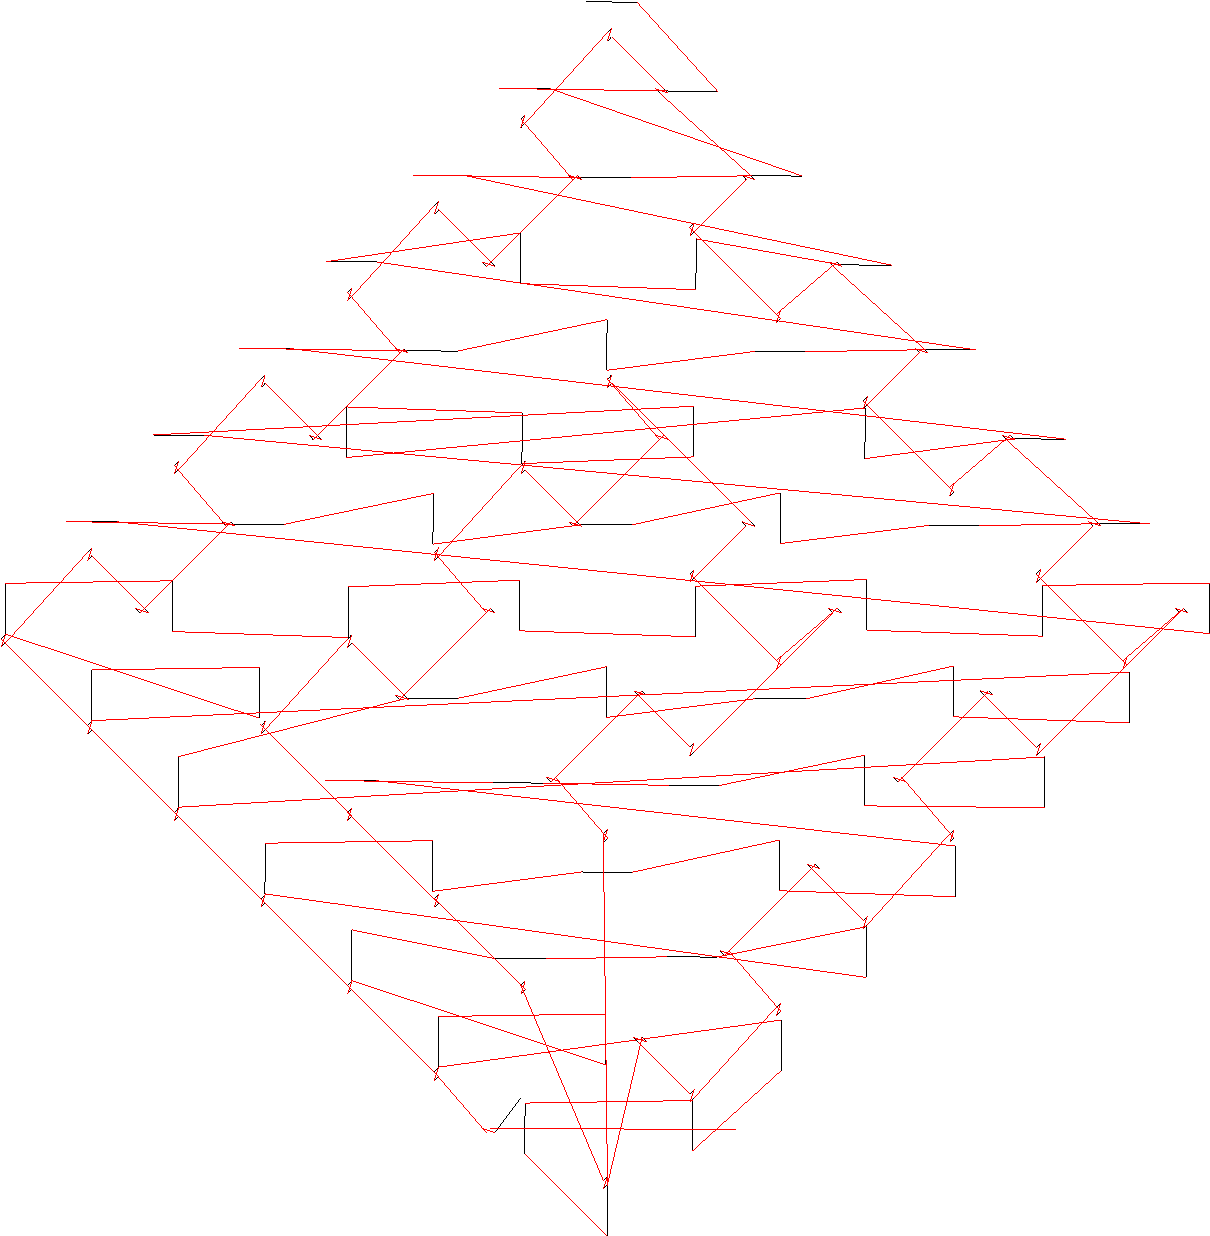
\includegraphics[width=0.32\textwidth]
    {sierpinski_print_yeahright_gcode-15-Abstract-Transitions.png}} 
    \subfigure[Optimiert -19\%]{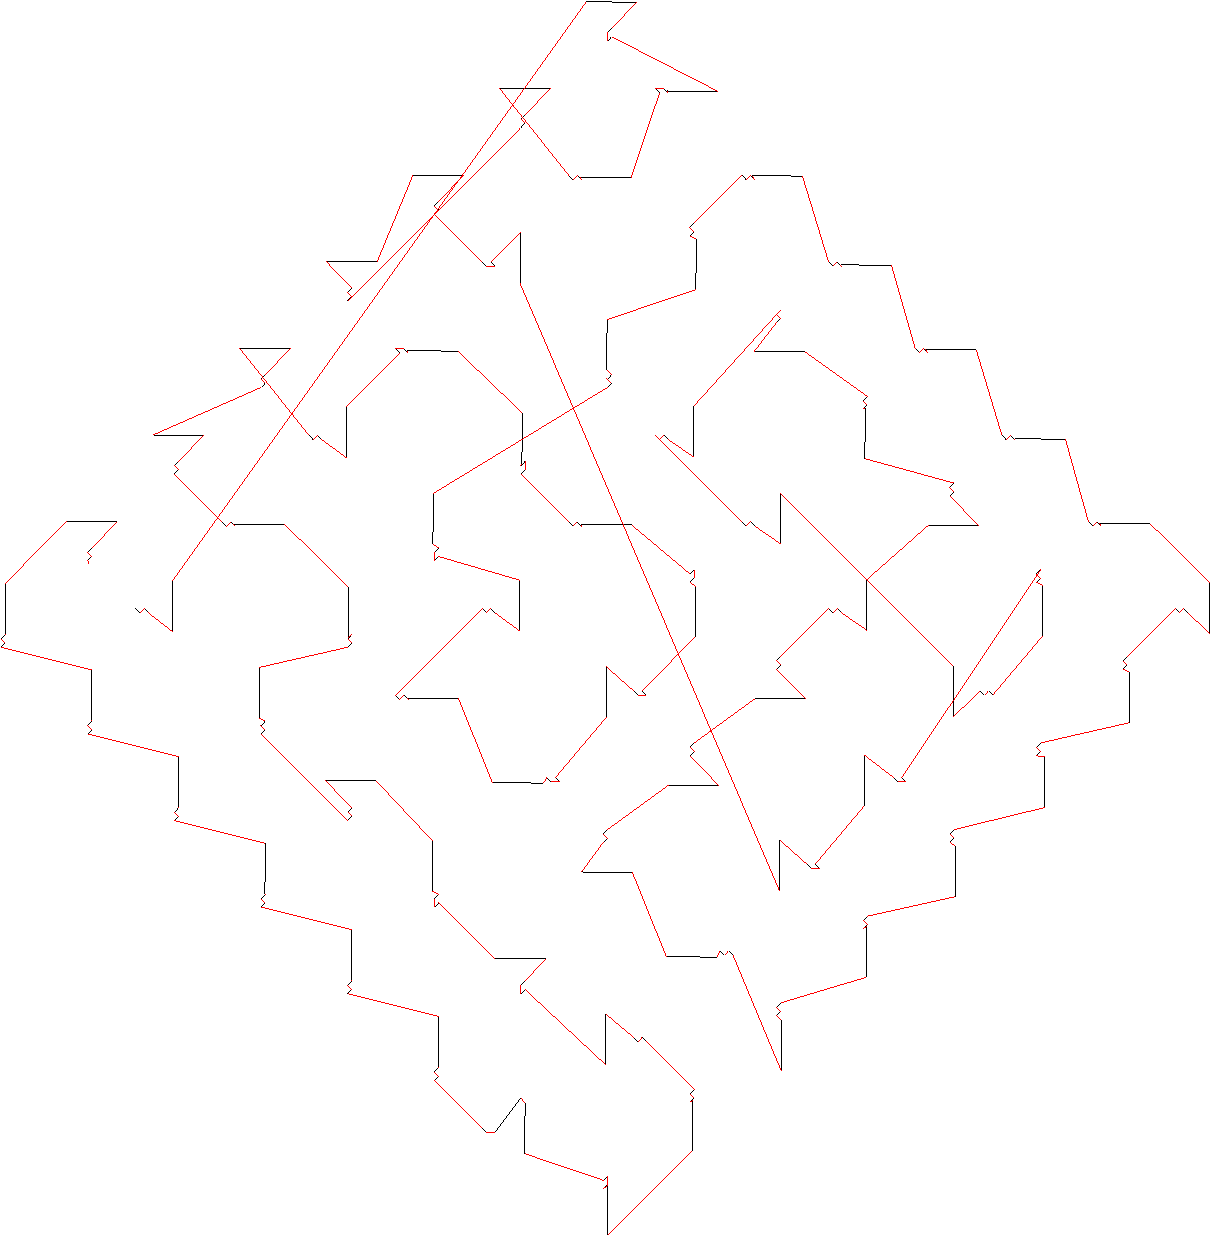
\includegraphics[width=0.32\textwidth]
    {sierpinski_print_yeahright_gcode-15-Abstract-Optimized-Transitions.png}} 
\caption[Schicht 15 aus dem Model \textit{Sierpinski Pyramide}\newline Screenshot erstellt mit unserem PrintOptimizer]{Schicht 15 aus dem Model \textit{Sierpinski Pyramide}} 
\label{img:sierpinski_layer}
\end{figure} 
%\begin{figure}[h!]
%    \subfigure[Druckpfad]{\includegraphics[width=0.25\textwidth]
%    {loubie_cat_body_and_pupils_v13_gcode-1-Full-NoTransitions.png}} 
%    \subfigure[Abstraktion]{\includegraphics[width=0.25\textwidth]
%    {loubie_cat_body_and_pupils_v13_gcode-1-Abstract-Transitions.png}} 
%    \subfigure[Optimiert -6\%]{\includegraphics[width=0.25\textwidth]
%    {loubie_cat_body_and_pupils_v13_gcode-1-Abstract-Optimized-Transitions.png}} 
%\caption{Schicht 1 aus dem Model \textit{Schrodinky}} 
%\label{img:schrodinky_layer}
%\end{figure} 
\end{samepage}

Man kann beim Vergleich der jeweiligen abstrahierten (b) und optimierten (c) Bildern in den Abbildungen \ref{img:benchy_layer} und \ref{img:sierpinski_layer} erkennen, dass die Transitionwege deutlich verkürzt und sinnvoller angeordnet sind. Die prozentuale Angabe bei (c) bezieht sich hier lediglich auf die Druckzeit des gezeigten Layers. Diese Verbesserungen lassen sich unter anderem durch die bereits in Kapitel \ref{kap:Problemstellung} erläuterten Eigenheiten des verwendeten Slicers erklären, da besonders beim Modell Sierpinski-Pyramide die Reihenfolge der Drucke einen großen Einfluss hat. Hier wird durch den Slicer zuerst jede Außenhaut der Quadrate gedruckt, anschließend alle Füllungen. Wir brechen diesen Ablauf jedoch auf, da wir nur zwischen Druck- und Transitionpfaden unterscheiden.


\newpage
\section{Fazit}
Durch das entwickelte Demoprogramm kann sehr gut dargestellt werden, dass viele Druckpfade nicht optimal (in Bezug auf die Pfadlänge) sind. Durch eine Verkürzung dieser Pfade kann die benötigte Dauer eines Drucks selbst mit einem naiven Algorithmus wie der \textit{Nearest Neighbour Selection} schon eine signifikante Zeitersparnis erreicht werden. Unsere Tests zeigen hier Verbesserungen zwischen 30 und 60 Prozent der originalen Transitionpfade, was im Mittel etwa 5 Prozent der gesamten Druckdauer einsparen kann. Diese Werte können durch Anwenden der in Kapitel \ref{kap:Heuristik} beschriebenen \textit{k-opt Heuristiken} nochmals verbessert werden. Da dieses Verfahren nicht trivial zu implementieren ist und wir mit unserem Ansatz schon deutlich machen konnten, dass es hier Optimierungsmöglichkeiten gibt, haben wir uns im Rahmen dieser Arbeit bewusst dagegen entschieden dieses Verfahren zusätzlich zu Implementieren. 
Dennoch haben wir während der Entwicklung großen Wert darauf gelegt, den Code ordentlich zu strukturieren um die Möglichkeit zu wahren auch später noch weitere Algorithmen oder Heuristiken implementieren zu können.

\newpage
\bibliographystyle{natdin}
\bibliography{Bibliography.bib}
\listoffigures

\end{document}